\documentclass[pra,aps,superscriptaddress,twocolumn]{revtex4-2}

\usepackage{amsmath}
\usepackage{amsfonts}
\usepackage{bm}
\usepackage{graphicx}
\usepackage{color}

\begin{document}

\title{Kolmogorov-Hinze scales in turbulent superfluids}

\author{Tsuyoshi Kadokura}
\affiliation{Department of Engineering Science, University of
Electro-Communications, Tokyo 182-8585, Japan}

\author{Hiroki Saito}
\affiliation{Department of Engineering Science, University of
Electro-Communications, Tokyo 182-8585, Japan}

\date{\today}

\begin{abstract}
When a two-component mixture of immiscible fluids is stirred, the fluids
are split into smaller domains with more vigorous stirring.
We numerically investigate the sizes of such domains in a stirred
two-component superfluid in a fully-developed turbulent state with
energy-input rate $\epsilon$.
For the strongly immiscible condition, the typical domain size is shown to
be proportional to $\epsilon^{-2/5}$, as predicted by the Kolmogorov-Hinze
theory in classical fluids.
For the weakly immiscible condition, quantum effects become pronounced and
the power changes from $-2 / 5$ to $-1 / 4$.
The domain size scaled by the interface thickness collapses into a universal
line.
\end{abstract}

\maketitle


When oil is poured into water and these fluids are stirred, the oil becomes
split into droplets in the water.
The droplet sizes become smaller with more vigorous stirring.
Such disintegration phenomena in multicomponent fluids are ubiquitous in
nature, and are important in engineering and industry.

Kolmogorov~\cite{Kolmogorov49} and Hinze~\cite{Hinze} considered the
disintegration process of droplets, and estimated the size of droplets in
turbulent fluids.
In fully-developed turbulence, the energy is input into the system as
large-scale eddies that cascade toward a smaller scale, resulting in the
Kolmogorov power law of the energy spectrum~\cite{Frisch}.
In such turbulent fluids, large-size droplets are unstable because they are
fragile to deformation and disintegration due to the fluctuating pressure
of the surrounding fluid.
Small droplets are thus produced by the breakup of large droplets, and this
breakup process continues to a scale where the turbulent energy to break
up the droplets becomes balanced with the droplet energy sustaining its
shape.
Droplets smaller than this scale coalesce into large droplets.
Therefore, there exists a characteristic size $D$ of droplets in turbulent
fluids, which is referred to as the Kolmogorov-Hinze (KH) scale, given
by~\cite{Hinze}
\begin{equation} \label{Hinze}
D \sim (\sigma / \rho)^{3/5} \epsilon^{-2/5},
\end{equation}
where $\sigma$ is the interface tension coefficient, $\rho$ is the density
of the surrounding fluid, and $\epsilon$ is the energy input rate to
maintain the turbulence.
The KH scale has been experimentally verified in various systems~\cite{Clay,Shinnar, Sleicher, Arai, Deane}.
Furthermore, direct numerical simulations have been performed over the last
decade~\cite{Perlekar12, Skartlien, Perlekar14, Fan, Perlekar17, Rosti}.

In this Letter, we extend the study of KH scales to a quantum mechanical
system: the superfluid turbulence of a two-component Bose-Einstein
condensate (BEC).
We will show that the KH scale also appears in this superfluid system and
is modified by quantum effects.
Turbulent behavior in superfluids has been widely studied.
For single-component superfluids, an isotropic fully-developed turbulent
state exhibits the Kolmogorov power law~\cite{Nore, Stalp, Araki,Kobayashi, Parker, Baggaley}.
The turbulent behavior of gaseous BECs has also been experimentally
studied~\cite{Henn, Neely, Kwon}, and a power law behavior has been observed
recently~\cite{Thompson, Navon, Johnstone, Navon2}.
A wide variety of systems have been studied theoretically, such as
two-dimensional systems~\cite{Nazarenko, Horng, Numasato, Bradley, Reeves},
dipolar superfluids~\cite{Bland}, and boundary layers~\cite{Stagg}.
Here, we focus on the turbulence in a two-component BEC.
Turbulence in multicomponent BECs has been investigated by many
researchers~\cite{Berloff, Takeuchi, Fujimoto, Tsubota, Vill, Kobyakov,
  Kang}.
In the context of domain-size scaling in multicomponent BECs, coarsening
dynamics following domain formation have been studied
extensively~\cite{Karl, Kudo, Hofmann, De, Nicklas, Williamson, Bourges,
  Prufer, Fujimoto18, Takeuchi18, Symes}.
However, the KH scale, i.e., domain-size scaling in conjunction with
the Kolmogorov turbulence, has not yet been investigated.

The KH scale in Eq.~(\ref{Hinze}) is derived as follows.
In a turbulent fluid, a domain undergoes fluctuating pressures that vary
over its size $D$, which causes deformation and disintegration of the
domain.
This pressure difference over the size $D$ can be expressed as $\sim \rho
v^2 \equiv P_{\rm turbulence}$, where $v$ is the velocity difference of the
surrounding fluid over the size $D$.
Within the inertial range of an isotropic homogeneous turbulence,
the statistical average of $v^2$ obeys the Kolmogorov two-thirds
law~\cite{Frisch}, $\bar{v^2} \propto (\epsilon D)^{2/3}$, and hence
$P_{\rm turbulence} \sim \rho (\epsilon D)^{2/3}$.
On the other hand, a domain tends to sustain its shape and resist
disintegration.
This sustaining force arises from the interface tension, and the pressure
required to deform the domain is thus estimated to be $\sim \sigma / D
\equiv P_{\rm sustain}$~\cite{Landau}. 
Breakup of domains to smaller sizes stops at the scale that satisfies
\begin{equation} \label{pp}
  P_{\rm sustain} \sim P_{\rm turbulence},
\end{equation}  
which gives the KH scale in Eq.~(\ref{Hinze}).

For an immiscible two-component BEC, the interface tension, which arises
from the interatomic interaction and quantum pressure, is well-defined, as
in classical fluids~\cite{Ao, Barankov, Schae}.
Therefore, we expect that the KH scale in Eq.~(\ref{Hinze}) also emerges in
two-component BECs when the thickness of the interface $W$ is much smaller
than the domain size $D$.
However, when $W$ is comparable to or larger than $D$, the picture of the
interface tension breaks down in the derivation of Eq.~(\ref{Hinze}).
The interface thickness $W$ is determined by the competition between the
quantum pressure and the intercomponent repulsion, and $W$ becomes large
when the former dominates the latter.
Thus, in the limit of large $W$, the mechanism to sustain domains against
disintegration originates mainly from the quantum pressure $P_{\rm sustain}
\sim \hbar^2 / (m D^2)$ instead of $P_{\rm sustain} \sim \sigma / D$, where
$m$ is the mass of an atom.
In this case, Eq.~(\ref{pp}) gives the characteristic size as
\begin{equation} \label{qHinze}
D \sim (\hbar / m)^{3/4} \epsilon^{-1/4}.
\end{equation}
Therefore, in the limit of weak segregation with large $W$, the quantum
mechanical effect becomes pronounced and the KH scale is expected to change
from the $-2/5$ to $-1/4$ power law with respect to $\epsilon$.
In the remainder of this Letter, we will corroborate this prediction using
numerical simulations of the coupled Gross-Pitaevskii (GP) equations.

In the mean-field approximation, a two-component BEC is described by the
coupled GP equations,
\begin{subequations}
\label{eq:BIN}
\begin{eqnarray}
			(i - \gamma)\hbar \frac{\partial \psi_1}{\partial t} & = & 
			\biggl(
				-\frac{\hbar^2}{2m}\nabla^2 + V_{\textrm{ext}}
			\nonumber \\
			& &
				+ g_{11}|\psi_1|^2 + g_{12}|\psi_2|^2 - \mu_1
			 \biggr) \psi_1,
			\\
			(i - \gamma)\hbar \frac{\partial \psi_2}{\partial t} & = & 
			\biggl(
				-\frac{\hbar^2}{2m}\nabla^2 + V_{\textrm{ext}}
				\nonumber \\
			& &
				+ g_{22}|\psi_2|^2 + g_{12}|\psi_1|^2 - \mu_2
			\biggr)\psi_2,
\end{eqnarray}
\end{subequations}
where $\psi_j(\bm{r}, t)$ is the macroscopic wave function of the $j$th
component, $V_{\rm ext}(\bm{r}, t)$ is the external stirring potential, and
$g_{jj'} = 4 \pi \hbar^2 a_{jj'} / m$ with $a_{jj'}$ being the $s$-wave
scattering length between the $j$th and $j'$th components.
The constant $\gamma$ in Eq.~(\ref{eq:BIN}) introduces dissipation of energy
from the condensate into thermal atoms~\cite{Choi}.
The value of $\gamma$ is selected in such a way that the energy dissipation
occurs predominantly below the scale of the healing length and does not
affect the dynamics in the inertial range.
The chemical potential $\mu_j$ is adjusted to maintain the unitarity, i.e.,
$\int |\psi_j|^2 d\bm{r}$ is conserved.

The miscibility between the two components is determined by the coupling
coefficients $g_{jj'}$.
The two superfluids are immiscible and phase separation occurs when
$g_{12}^2 > g_{11} g_{22}$ is satisfied~\cite{Pethick}.
In the following, we assume $g_{11} = g_{22} \equiv g > 0$ and $g_{12} > 0$;
therefore, the immiscible condition reduces to
\begin{equation} \label{im}
g_{12} > g.
\end{equation}
The phase separation of immiscible components produces an interface, at
which excess energy arises, resulting in the interface tension.
For $g_{12} / g - 1 \ll 1$, the interface tension coefficient is
given by~\cite{Ao, Barankov, Schae}
\begin{equation} \label{sigma}
\sigma \simeq \left[ \frac{\hbar^2 n^3}{2m} (g_{12} - g) \right]^{1/2},
\end{equation}
where $n$ is the number density far from the interface.
The thickness $W$ of the interface between two components, over which each
density changes from 0 to $n$ (or $n$ to 0), has the form
\begin{equation} \label{W}
W \simeq \xi (g_{12} / g - 1)^{-1/2},
\end{equation}
where $\xi = \hbar / (2mgn)^{1/2}$ is the healing length.

\begin{figure}[t]
	\includegraphics[width=8.5cm]{fig1.eps}
 	\caption{
    A two-component BEC is stirred by a plate-shaped potential (red or black)
    to generate a turbulent state.
		(a) Snapshot of a fully-developed turbulent state at $t = 2000$ for
    $g' \equiv g_{12} / g = 1.02$ and $\nu_{\rm plate} = 0.0048$.
		Isodensity surfaces of $|\psi_1|^2 = 0.5$ (purple or dark gray) and
    $|\psi_2|^2 = 0.5$ (green or light gray) are shown.
    The arrow indicates the range of sinusoidal motion of the stirring
    potential.
		(b)-(c) Cross-sectional views of $|\psi_1|^2$ and $|\psi_1|^2 +
    |\psi_2|^2$ at $z=32$.
    The arrows indicate the direction of the potential motion.
		(d) Energy spectra $E(k)$ (arbitrary unit) for $\gamma = 0.01, 0.03$, and
    $0.05$, averaged over $t = 1900$-$2000$.
		The dashed line has a slope of $-5/3$.
		See the Supplemental Material for a movie of the dynamics~\cite{SM}.
	}
	\label{f:setup}
\end{figure}
The length, time, and wave functions are normalized by $\xi$, $\hbar /
(gn)$, and $\sqrt{n}$, respectively, where $n$ is taken to be an average
density of each component.
In this unit, the interaction coefficients appear in the normalized GP
equation only through $g_{12} / g \equiv g'$.
We consider a box of size $L^3=64^3$ with a periodic boundary condition, in
which the two components are equally populated, $\int |\psi_1|^2 d\bm{r} =
\int |\psi_2|^2 d\bm{r} = L^3$.
To generate the turbulent state, the system is stirred by a plate-shaped
potential $V_{\textrm{ext}}$ with a size of $1 \times 32 \times 64$ and a
potential height of $10$.
This plate-shaped potential is moved sinusoidally over the system ($0 < x <
L$) at a frequency $\nu_{\rm plate}$, as shown in Fig.~\ref{f:setup}(a),
which can input the turbulent energy into the large scale.
The coupled GP equations (\ref{eq:BIN}) are numerically solved using the
pseudospectral method~\cite{Recipe}.
The space is discretized into a $128^3$ mesh and the time step is typically
$10^{-3}$.
The initial state has uniform density with random phases on each mesh.

The two-component BEC is stirred until the fully-developed turbulent state
is achieved.
Figure~\ref{f:setup}(a) shows isodensity surfaces of $|\psi_1|^2$ and
$|\psi_2|^2$ at $t = 2000$ for $g' = 1.02$ and $\nu_{\rm plate} = 0.0048$.
The immiscible condition (\ref{im}) is satisfied for this value of $g'$;
therefore, the two components are separated and domains are formed in
each component.
Figure~\ref{f:setup}(a) shows that the domain sizes are typically
$\gtrsim 10$, while $W \simeq (1.02 - 1)^{-1/2} \simeq 7$ from Eq.~(\ref{W}).
The KH scale is thus expected to be marginally in the region of
Eq.~(\ref{Hinze}) (rather than Eq.~(\ref{qHinze})) with this condition,
which will be investigated later.
Figures~\ref{f:setup}(b) and \ref{f:setup}(c) show cross-sectional views of
the densities $|\psi_1|^2$ and $|\psi_1|^2 + |\psi_2|^2$, respectively,
where the stirring potential is moving rightward at this moment.
Although the density $|\psi_1|^2$ (or $|\psi_2|^2$) largely varies in space
due to the phase separation (Fig.~\ref{f:setup}(b)), the total density far
from the stirring potential is almost uniform (Fig.~\ref{f:setup}(c)).
The small density holes in Fig.~\ref{f:setup}(c) indicate that quantized
vortices are generated behind the potential moving at almost the sound
velocity of the density wave.
To confirm that the system has reached the Kolmogorov turbulence, we
calculate the energy spectrum $E(k)$ of incompressible velocity
field~\cite{Nore} averaged over the duration of $t = 1900$-2000 for
$\gamma = 0.01$, 0.03, and 0.05, which is shown in Fig.~\ref{f:setup}(d).
The slope of the logarithmic plot of $E(k)$ agrees well with the Kolmogorov
power law of $-5 / 3$ within the inertial range of the wave number ($k
\lesssim 2$).
In this range, the lines in Fig.~\ref{f:setup}(d) are almost independent of
the dissipation constant $\gamma$, which indicates that, for these values of
$\gamma$, the energy dissipation occurs predominantly at the small length
scale and does not affect the dynamics in the inertial range.
In the following calculations, we take $\gamma = 0.03$.

\begin{figure}[t]
	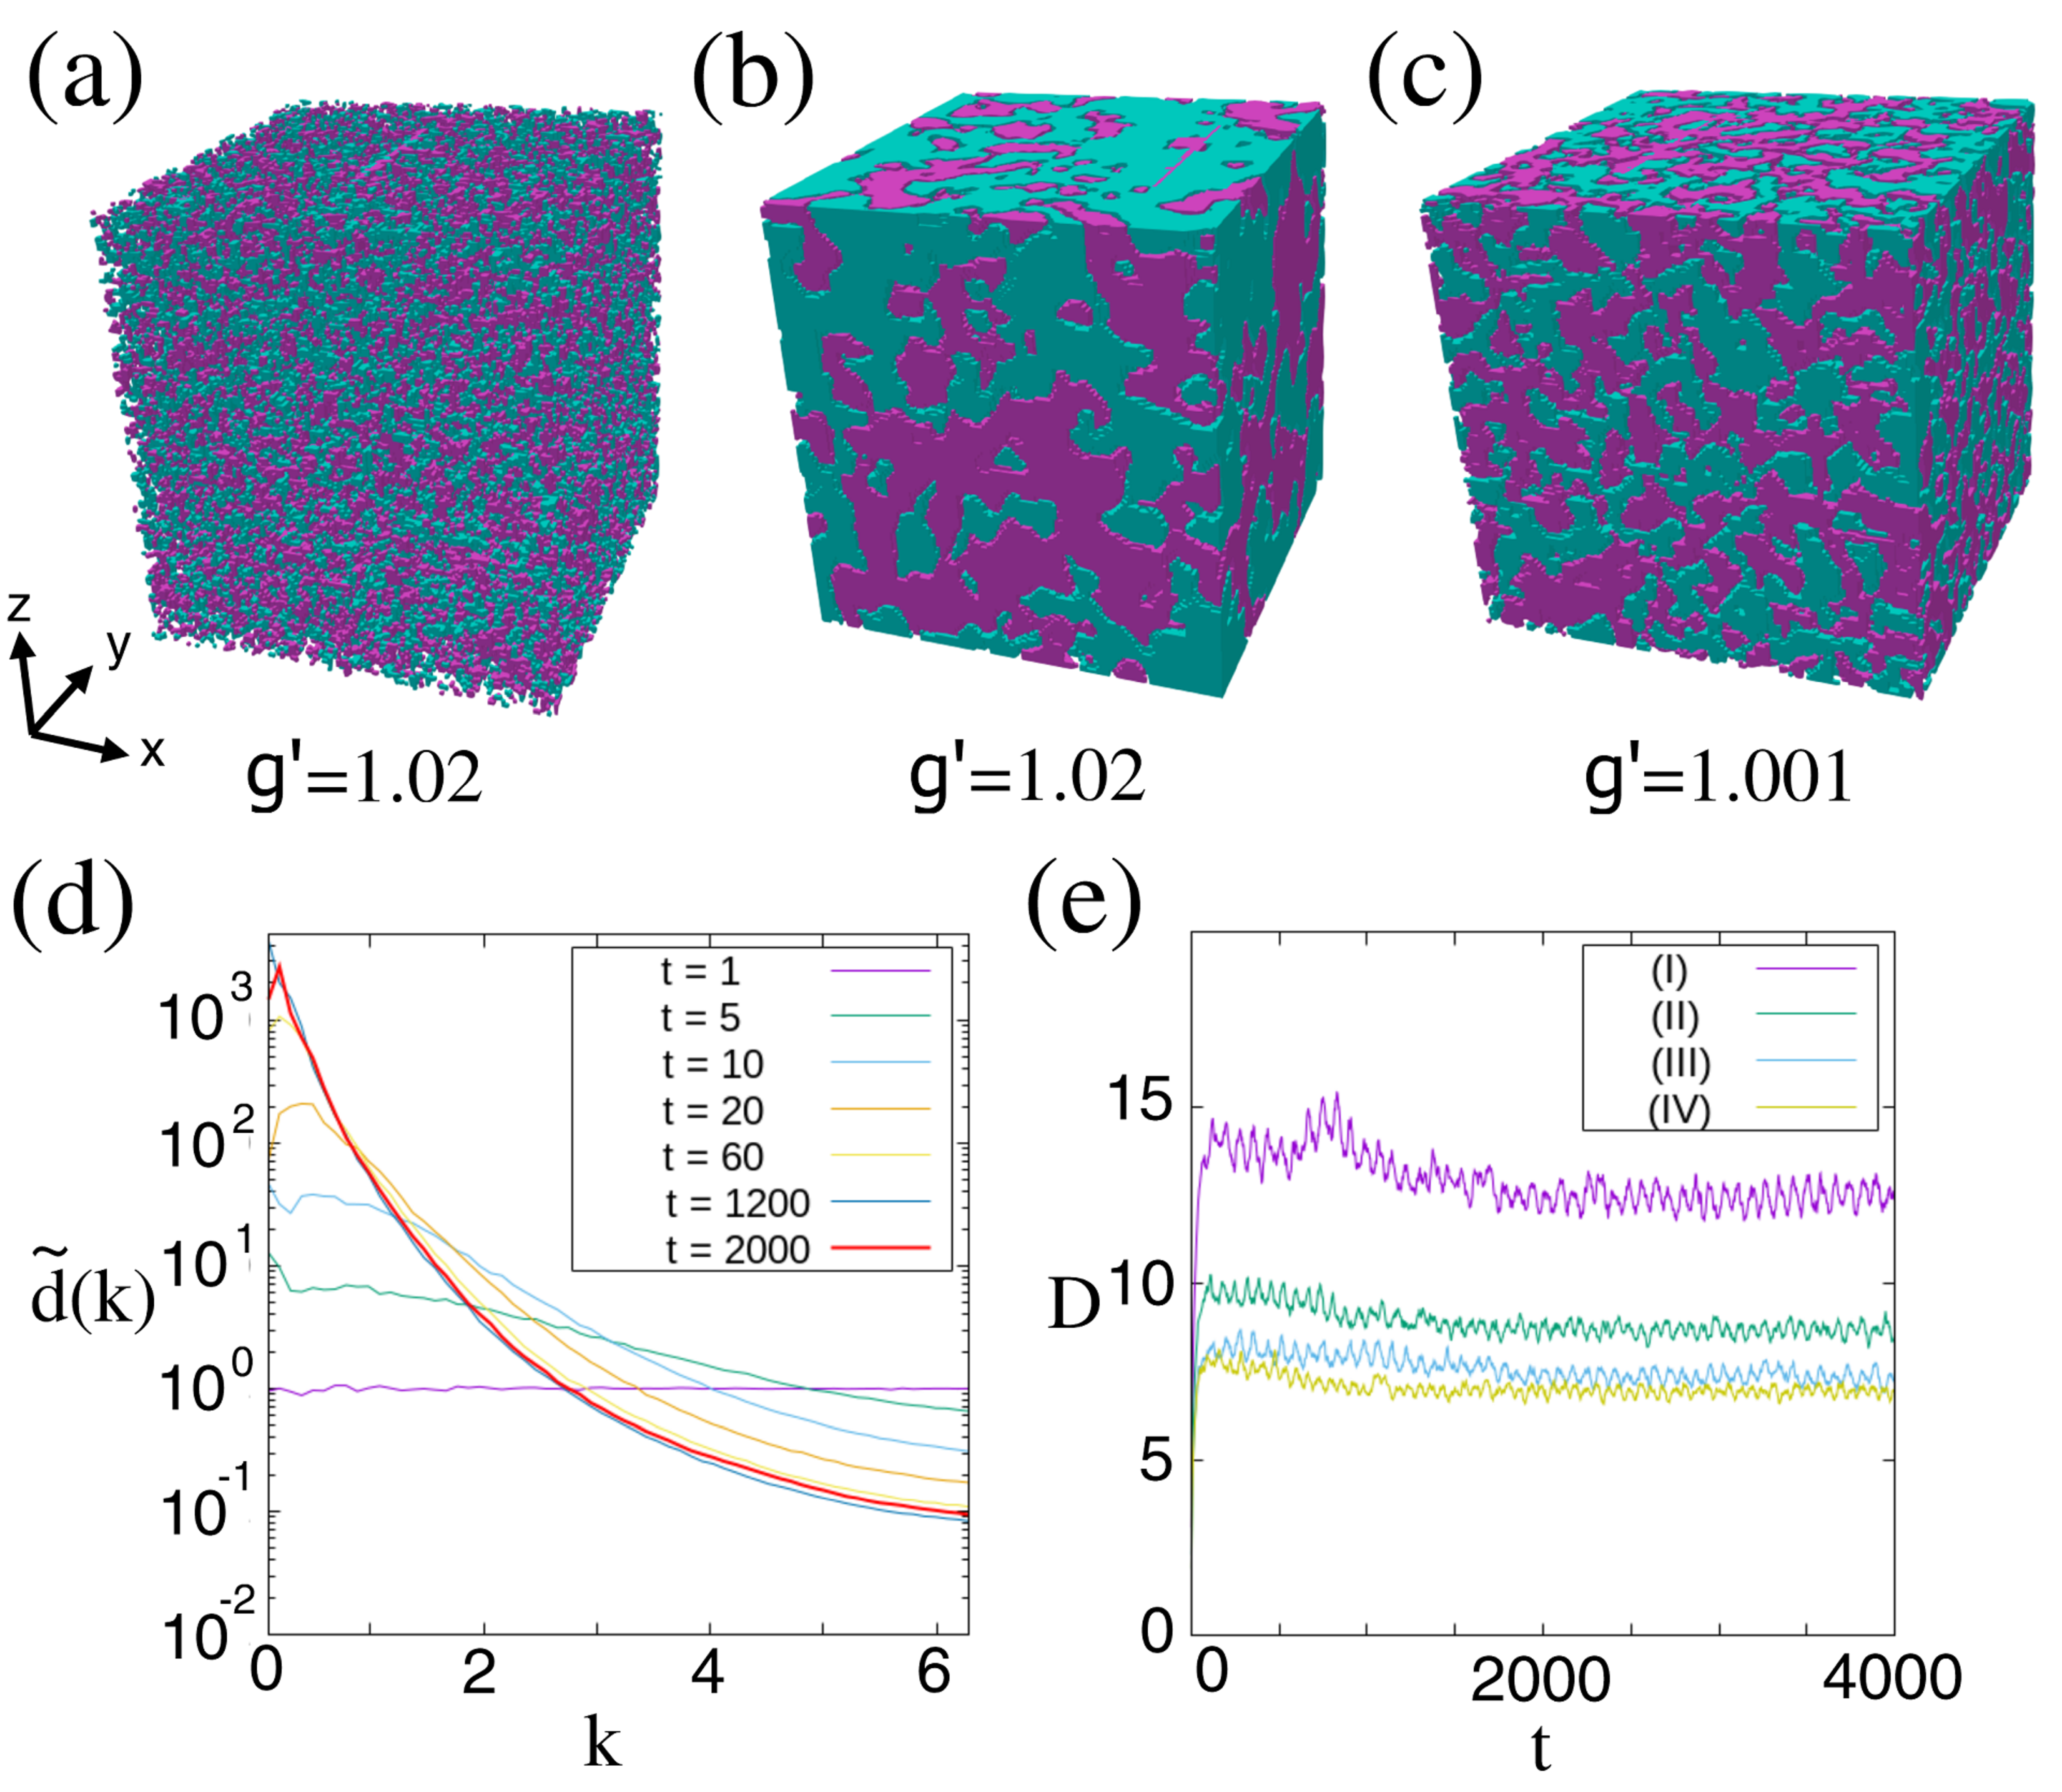
\includegraphics[width=9cm]{fig2.eps}
	\caption{
		Discretized density distributions $d(\bm{r})$ in Eq.~(\ref{d}) at
    (a) $t = 1$ for $g' \equiv g_{12} / g = 1.02$,
    (b) $t = 2000$ for $g' = 1.02$, and
		(c) $t = 2000$ for $g' = 1.001$.	
	  (d) Time development of the radial wave-number distribution
    $\tilde d(k)$ for $g' = 1.02$.
    In (a)-(d), $\nu_{\rm plate} = 0.0048$.
		(e) Time development of the typical domain size $D \equiv 2\pi / [\int k
      \tilde d(k) dk / \int \tilde d(k) dk]$ for $(g', \nu_{\rm plate}) =
    (1.02, 0.0032)$, $(1.02, 0.0048)$, $(1.01, 0.0048)$, and
    $(1.001, 0.0048)$, which are labeled as (I), (II), (III), and (IV),
    respectively.
	}
	\label{f:arrest}
\end{figure}
The following procedure is used to numerically evaluate the typical size of
the domains.
We first discretize the density-imbalance distribution as
\begin{equation} \label{d}
  d(\bm{r}) = \left\{
  \begin{array}{ll}
    1 & (|\psi_1(\bm{r})|^2 \geq |\psi_2(\bm{r})|^2) \\
    -1 & (|\psi_1(\bm{r})|^2 < |\psi_2(\bm{r})|^2),
  \end{array} \right.
\end{equation}
which eliminates the information of the interface thickness and small
excitations, and enables the information of only the domain size to be
extracted.
Figures~\ref{f:arrest}(a)-\ref{f:arrest}(c) show snapshots of the
distributions of $d(\bm{r})$.
Fourier transformation of $d(\bm{r})$ is performed and its azimuthal average
in the $\bm{k}$ space is taken, which we denote as $\tilde d(k)$.
Figure~\ref{f:arrest}(d) shows the time evolution of $\tilde d(k)$ for the
dynamics in Fig.~\ref{f:setup}.
Since the initial state has a random phase on each mesh, $\tilde d(k)$ is
initially independent of $k$.
The distribution of $\tilde d(k)$ then tilts toward small wave numbers, and
the steady distribution is reached for $t \gtrsim 1200$.
We have confirmed that the steady distribution of $\tilde d(k)$ does not
depend on the initial state.
The first moment of $\tilde d(k)$, $\int k \tilde d(k) dk / \int \tilde d(k)
dk \equiv \langle k \rangle$, gives a typical wave number in the density
distribution, and thus $2\pi / \langle k \rangle \equiv D$ characterizes the
size of the domains.
Figure~\ref{f:arrest}(e) shows the time development of $D$ for different
values of $g'$ and $\nu_{\rm plate}$.
The size $D$ in the steady state decreases with $g'$ and with an increase in
$\nu_{\rm plate}$.
This is because the interface tension (\ref{sigma}) decreases with $g'$ and
the energy input rate increases with $\nu_{\rm plate}$.

To study the KH scale quantitatively, we need to calculate the rate
$\epsilon$ at which the energy is input into the system by the stirring
potential.
Let the position of the plate-shaped potential be $x_{\rm plate}(t)$, which
moves in the $\pm x$ direction, as shown in Fig.~\ref{f:setup}.
The force acting on the potential from the superfluid is then
$F = -\partial / (\partial x_{\rm plate}) \int
V_{\rm ext}(\bm{r}; x_{\rm plate}) [|\psi_1(\bm{r})|^2 + |\psi_2(\bm{r})|^2]
d\bm{r}$.
The energy input rate is thus given by $\epsilon = -F \dot x_{\rm plate}$.
The value of $\epsilon$ (and also $D$) fluctuates in time due to the random
nature of the turbulence.
The sinusoidal motion of the plate-shaped potential also causes periodic
fluctuation, as shown in Fig.~\ref{f:arrest}(e).
Therefore, we take the temporal average of these quantities, $\bar\epsilon$
and $\bar D$, over a sufficiently long time after the steady turbulent state
is achieved.
The inset in Fig.~\ref{f:hinze}(a) shows $\bar\epsilon$ as a function of
$\nu_{\rm plate}$ for $g' = 1.02$ and 1.001.

\begin{figure}[t]
	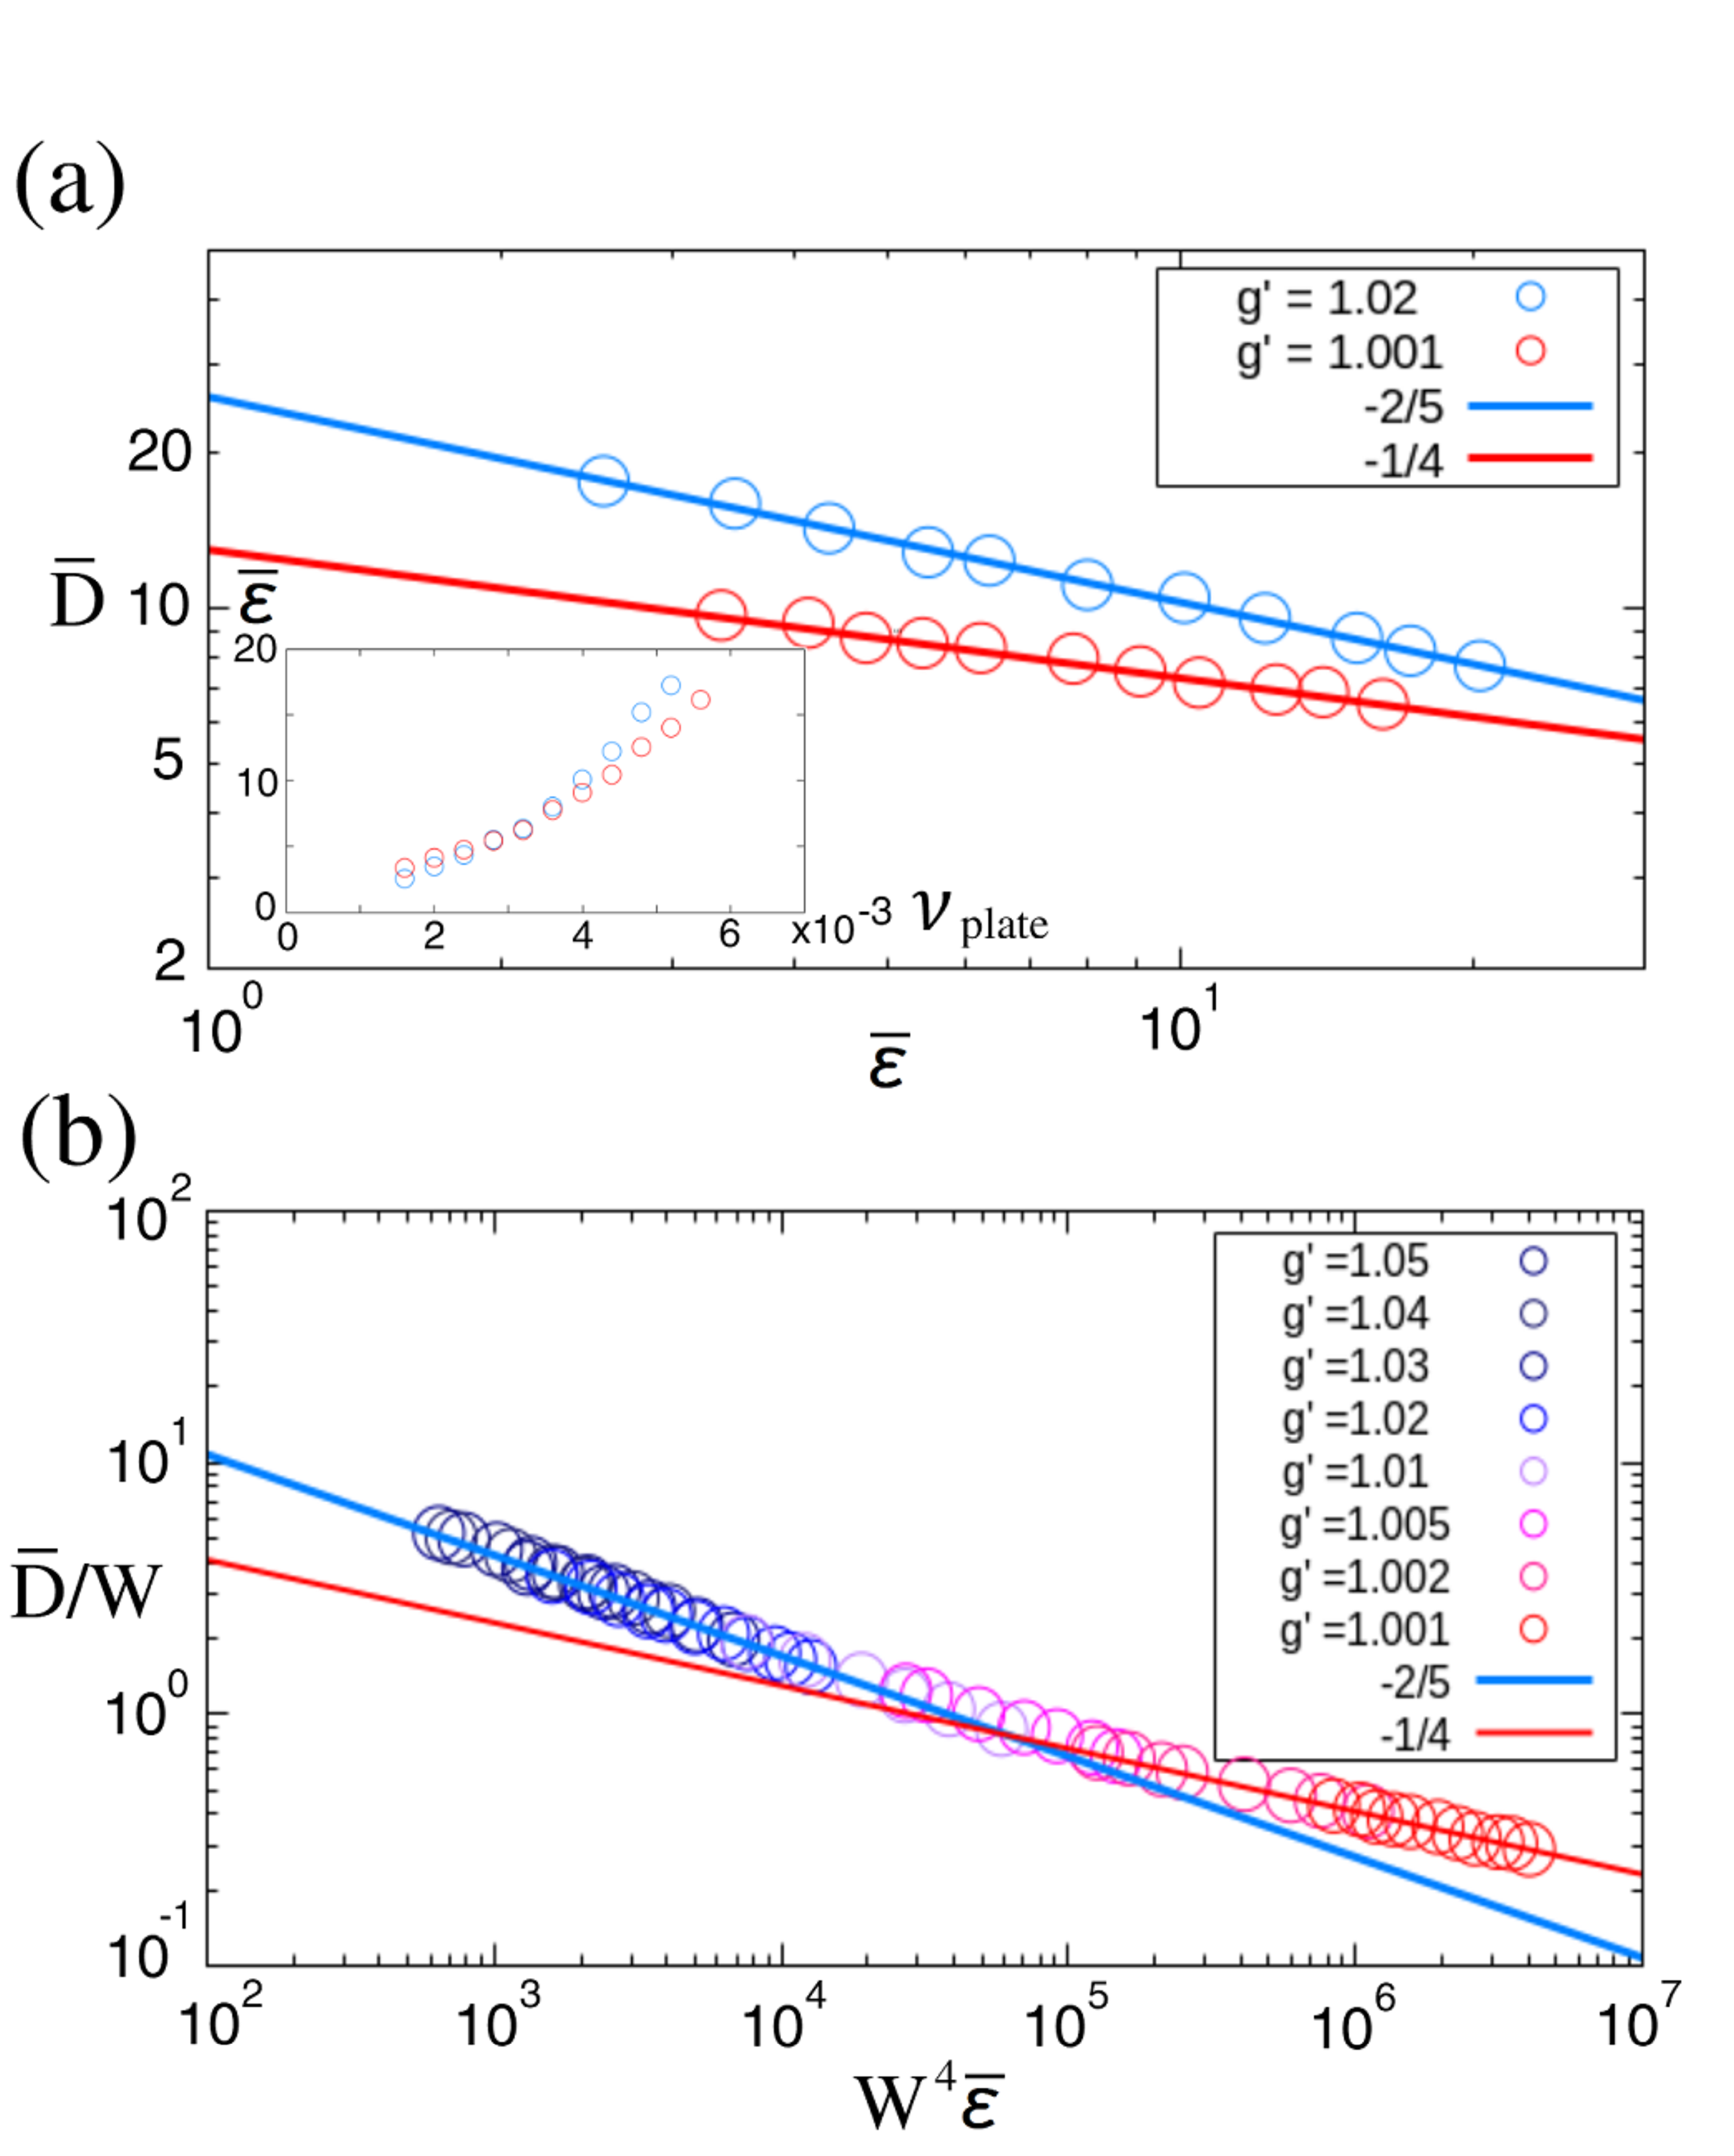
\includegraphics[width=8cm]{fig3.eps}
	\caption{
		(a) Typical domain size $\bar D$ versus energy-input rate $\bar\epsilon$
    for the steady turbulent state with $g' \equiv g_{12} / g = 1.02$ and
    1.001.
    The slopes of the lines are $-2/5$ and $-1/4$ for comparison with
    Eqs.~(\ref{Hinze}) and (\ref{qHinze}).
    The inset shows $\bar\epsilon$ as a function of $\nu_{\rm plate}$.
    (b) $\bar D$ and $\bar\epsilon$ are rescaled with respect to the
    interface width $W$ for various values of $g'$.
    The plots collapse into a universal curve.
    The slopes of the lines are $-2/5$ and $-1/4$.
	}
	\label{f:hinze}
\end{figure}
Now we are ready to investigate the KH scales in a turbulent superfluid in
the classical and quantum regimes, as given in Eqs.~(\ref{Hinze}) and
(\ref{qHinze}).
The result is shown in Fig.~\ref{f:hinze}, which is the main result of this
work.
Figure~\ref{f:hinze}(a) plots the typical domain size $\bar D$ versus the
energy-input rate $\bar\epsilon$ for $g' = 1.02$ and 1.001.
For $g' = 1.02$, the plots obey the power law $\propto \bar\epsilon^{-2/5}$,
which agrees with the classical KH scale in Eq.~(\ref{Hinze}).
This implies that the two components are well separated, and the mechanism
that sustains the domains against disintegration can be described by the
interface tension in this region.
%In fact, $\bar D \gtrsim 10$ in Fig.~\ref{f:hinze}(a) is larger than $W =
%(1.02 - 1)^{-1/2} \simeq 7$.
For $g' = 1.001$, on the other hand, the plots in
Fig.~\ref{f:hinze}(a) follow the power law $\propto \bar\epsilon^{-1/4}$,
which agrees with the KH scale in the quantum region in Eq.~(\ref{qHinze}),
implying that the mechanism to sustain domains is mainly the quantum
kinetic pressure arising from the uncertainty principle.
In this region, $\bar D \lesssim 10$ is smaller than
$W \simeq (1.001 - 1)^{-1/2} \simeq 32$ and the interface tension of domains
is not well-defined.

As discussed in deriving Eqs.~(\ref{Hinze}) and (\ref{qHinze}), and
numerically confirmed in Fig.~\ref{f:hinze}(a), the different power laws
emerge, depending on the two length scales: the domain size $\bar D$ and the
interface width $W = (g' - 1)^{-1/2}$.
Therefore, we use the rescaled domain size, $\bar D / W$.
We can deduce that the crossover between the two power laws,
Eqs.~(\ref{Hinze}) and (\ref{qHinze}), always lies in the region of
$\bar D / W \sim 1$. 
Note that Eq.~(\ref{qHinze}) does not include $W$, and therefore, in the
quantum KH region, $\bar D = c \bar\epsilon^{-1/4}$ can be rewritten as
$\bar D / W = c (W^4 \bar\epsilon)^{-1/4}$ with a coefficient $c$ that is
independent of $W$.
The $\bar D / W$ versus $W^4 \bar\epsilon$ line is thus universal in the
region of the $-1/4$ power law, and the crossover to the region of the
$-2/5$ power law always occurs at $\bar D / W \sim 1$; therefore it is
expected that this line is universal over the entire region.
Figure~\ref{f:hinze}(b) plots $\bar D / W$ versus $W^4 \bar\epsilon$ for
various values of $g'$.
As expected, all the plots collapse into the universal curve, which bridges
the two regions of the $-2/5$ and $-1/4$ power laws.
Although $\bar D$ and $\bar\epsilon$ are restricted to narrow ranges for
each value of $g'$ in the present numerical simulations, the rescaled plot
in Fig.~\ref{f:hinze}(b) significantly extends the effective ranges of $\bar
D$ and $\bar\epsilon$, which corroborates the existence of the two power
laws in the superfluid KH scale.

Finally, we discuss the possible experimental realization of the present
result.
A box potential will be suitable to avoid complexity arising from the
inhomogeneous $|\psi_1|^2 + |\psi_2|^2$ distribution in a harmonic
potential.
The stirring potential can be produced by a far-off-resonant laser beam.
Shaking of an optical box can also be used to generate the turbulent
state~\cite{Navon}.
The typical size of the domains can be inferred from the imaging data, where
the slice imaging of a three-dimensional distribution may be
required~\cite{Andrews}.
It is difficult to measure the energy input rate directly; therefore, the
support of numerical simulation is necessary, which provides the relation
between the motion of the potential and the energy input rate, as in the
inset in Fig.~\ref{f:hinze}(a).
The interaction $g_{12}$ can be varied using the Feshbach resonance
technique.

In conclusion, we have investigated the KH scale of domain sizes in
immiscible two-component superfluids in a fully-developed turbulent state.
We predict that two regions of the KH scale exist with different power
laws, which reflect the quantum property of the system.
Numerical simulations of the coupled GP equations were performed, and the
typical domain size $D$ was confirmed to obey the power laws with respect to
the energy input rate $\epsilon$.
We found the universal function of the rescaled quantities $D / W$ and
$W^4 \epsilon$, which connects the two regions of the quantum and
classical KH scales.
A possible extension of this study is a three-component system, in which the
third component can change the interface tension of the other two
components, resulting in emulsification.

This work was supported by JSPS KAKENHI Grant Number JP20K03804.



\begin{thebibliography}{99}

\bibitem{Kolmogorov49}
A. N. Kolmogorov,
%On the breakage of drops in a turbulent flow,
Dokl. Akad. Nauk. SSSR \textbf{66}, 825 (1949).

\bibitem{Hinze}
J. O. Hinze,
%Fundamentals of the Hydrodynamic Mechanism of Splitting in Dispersion Process,
AIChE J. \textbf{1}, 289 (1955).

\bibitem{Frisch}
See, e.g., U. Frisch, {\it Turbulence: The Legacy of A. N. Kolmogorov}
(Cambridge University Press, Cambridge, UK, 1995).

\bibitem{Clay}
P. H. Clay,
%The mechanism of emulsion formation in turbulent flow,
Proc. Roy. Acad. Sci. (Amsterdam) \textbf{43}, 852 (1940).    

\bibitem{Shinnar}
R. Shinnar,
%On the behaviour of liquid dispersions in mixing vessels,
J. Fluid Mech. \textbf{10}, 259 (1961).

\bibitem{Sleicher}
C. A. Sleicher,
%Maximum Stable Drop Size in Turbulent Flow,
AIChE J. \textbf{8}, 471 (1964).

\bibitem{Arai}
K. Arai, M. Konno, Y. Matunaga, and S. Saito,
%EFFECT OF DISPERSED-PHASE VISCOSITY ON THE MAXIMUM STABLE DROP SIZE FOR
%BREAKUP IN TURBULENT FLOW
J. Chem. Eng. Jpn. \textbf{10}, 325 (1977).

\bibitem{Deane}
G. B. Deane and M. D. Stokes, 
%Scale dependence of bubble creation mechanisms in breaking waves,
Nature (London) \textbf{418}, 839 (2002).

\bibitem{Perlekar12}
P. Perlekar, L. Biferale, M. Sbragaglia, S. Srivastava, and F. Toschi,
%Droplet size distribution in homogeneous isotropic turbulence,
Phys. Fluids \textbf{24}, 065101 (2012).

\bibitem{Skartlien}
R. Skartlien, E. Sollum, and H. Schumann,
%Droplet size distributions in turbulent emulsions: Breakup criteria and
%surfactant effects from direct numerical simulations,
J. Chem. Phys. \textbf{139}, 174901 (2013).

\bibitem{Perlekar14}
P. Perlekar, R. Benzi, H. J. H. Clercx, D. R. Nelson, and F. Toschi,
%Spinodal Decomposition in Homogeneous and Isotropic Turbulence,
Phys. Rev. Lett. \textbf{112}, 014502 (2014).

\bibitem{Fan}
X. Fan, P. H. Diamond, L. Chac\'on, and H. Li,
%Cascades and spectra of a turbulent spinodal decomposition
%in two-dimensional symmetric binary liquid mixtures,
Phys. Rev. Fluids \textbf{1}, 054403 (2016).
  
\bibitem{Perlekar17}
P. Perlekar, N. Pal, and R. Pandit,
%Two-dimensional Turbulence in Symmetric Binary-Fluid Mixtures:
%Coarsening Arrest by the Inverse Cascade,
Sci. Rep. \textbf{7}, 44589 (2017).

\bibitem{Rosti}
M. E. Rosti, Z. Ge, S. S. Jain, M. S. Dodd, and L. Brandt,
%Droplets in homogeneous shear turbulence,
J. Fluid Mech. \textbf{876}, 962 (2019).

\bibitem{Nore}
C. Nore, M. Abid, and M. E. Brachet,
%Kolmogorov Turbulence in Low-Temperature Superflows,
Phys. Rev. Lett. \textbf{78}, 3896 (1997);
%Decaying Kolmogorov turbulence in a model of superflow,  
Phys. Fluids \textbf{9}, 2644 (1997).

\bibitem{Stalp}
S. R. Stalp, L. Skrbek, and R. J. Donnelly,
%Decay of Grid Turbulence in a Finite Channel,
Phys. Rev. Lett. \textbf{82}, 4831 (1999).

\bibitem{Araki}
T. Araki, M. Tsubota, and S. K. Nemirovskii,
%Energy Spectrum of Superfluid Turbulence with No Normal-Fluid Component,
Phys. Rev. Lett. \textbf{89}, 145301 (2002).

\bibitem{Kobayashi}
M. Kobayashi and M. Tsubota,
%Kolmogorov Spectrum of Superfluid Turbulence: Numerical Analysis
%of the Gross-Pitaevskii Equation with a Small-Scale Dissipation,
Phys. Rev. Lett. \textbf{94}, 065302 (2005).

\bibitem{Parker}
N. G. Parker and C. S. Adams,
%Emergence and Decay of Turbulence in Stirred Atomic Bose-Einstein
%Condensates,
Phys. Rev. Lett. \textbf{95}, 145301 (2005).

\bibitem{Baggaley}
A. W. Baggaley, J. Laurie, and C. F. Barenghi,
%Vortex-Density Fluctuations, Energy Spectra, and Vortical Regions in
%Superfluid Turbulence,  
Phys. Rev. Lett. \textbf{109}, 205304 (2012).

\bibitem{Henn}
E. A. L. Henn, J. A. Seman, G. Roati, K. M. F. Magalh\~aes, and V. S. Bagnato,
%Emergence of Turbulence in an Oscillating Bose-Einstein Condensate,  
Phys. Rev. Lett. \textbf{103}, 045301 (2009).

\bibitem{Neely}
T. W. Neely, A. S. Bradley, E. C. Samson, S. J. Rooney, E. M. Wright,
K. J. H. Law, R. Carretero-Gonz\'alez, P. G. Kevrekidis, M. J. Davis, and
B. P. Anderson,
%Characteristics of Two-Dimensional Quantum Turbulence in a Compressible
%Superfluid,
Phys. Rev. Lett. \textbf{111}, 235301 (2013).

\bibitem{Kwon}
W. J. Kwon, G. Moon, J.-Y. Choi, S. W. Seo, Y.-I. Shin,
%Relaxation of superfluid turbulence in highly oblate Bose-Einstein
%condensates,  
Phys. Rev. A \textbf{90}, 063627 (2014).

\bibitem{Thompson}
K. J. Thompson, G. G. Bagnato, G. D. Telles, M. A. Caracanhas, F. E. A. dos
Santos, and V. S. Bagnato,
%Evidence of power law behavior in the momentum distribution of a turbulent
%trapped Bose-Einstein condensate,
Laser Phys. Lett. \textbf{11}, 015501 (2014).

\bibitem{Navon}
N. Navon, A. L. Gaunt, R. P. Smith, and Z. Hadzibabic,
%Emergence of a turbulent cascade in a quantum gas,
Nature (London) \textbf{539}, 72 (2016).

\bibitem{Johnstone}
S. P. Johnstone, A. J. Groszek, P. T. Starkey, C. J. Billington,
T. P. Simula, and K. Helmerson,
%Evolution of large-scale flow from turbulence in a two-dimensional
%superfluid
Science \textbf{364}, 1267 (2019).

\bibitem{Navon2}
N. Navon, C. Eigen, J. Zhang, R. Lopes, A. L. Gaunt, K. Fujimoto,
M. Tsubota, R. P. Smith, and Z. Hadzibabic,
Science \textbf{366}, 382 (2019).

\bibitem{Nazarenko}
S. Nazarenko and M. Onorato,
%Freely decaying Turbulence and Bose-Einstein Condensation in
%Gross-Pitaevski Model  
J. Low Temp. Phys. \textbf{146}, 31 (2007).

\bibitem{Horng}
T.-L. Horng, C.-H. Hsueh, S.-W. Su, Y.-M. Kao, and S.-C. Gou,
%Two-dimensional quantum turbulence in a nonuniform Bose-Einstein condensate
Phys. Rev. A \textbf{80}, 023618 (2009).

\bibitem{Numasato}
R. Numasato, M. Tsubota, and V. S. L'vov,
%Direct energy cascade in two-dimensional compressible quantum turbulence
Phys. Rev. A \textbf{81}, 063630 (2010).

\bibitem{Bradley}
A. S. Bradley and B. P. Anderson,
%Energy Spectra of Vortex Distributions in Two-Dimensional Quantum
%Turbulence  
Phys. Rev. X \textbf{2}, 041001 (2012).

\bibitem{Reeves}
M. T. Reeves, T. P. Billam, B. P. Anderson, and A. S. Bradley,
%Inverse Energy Cascade in Forced Two-Dimensional Quantum Turbulence
Phys. Rev. Lett. \textbf{110}, 104501 (2013).

\bibitem{Bland}
T. Bland, G. W. Stagg, L. Galantucci, A. W. Baggaley, and N. G. Parker,
%Quantum Ferrofluid Turbulence  
Phys. Rev. Lett. \textbf{121}, 174501 (2018).

\bibitem{Stagg}
G. W. Stagg, N. G. Parker, and C. F. Barenghi,
%Superfluid Boundary Layer  
Phys. Rev. Lett. \textbf{118}, 135301 (2017).

\bibitem{Berloff}
N. G. Berloff and C. Yin,
%Turbulence and Coherent Structures in Two-Component Bose Condensates,
J. Low Temp. Phys. \textbf{145}, 187 (2006).

\bibitem{Takeuchi}
H. Takeuchi, S. Ishino, and M. Tsubota,
%Binary Quantum Turbulence Arising from Countersuperflow Instability in
%Two-Component Bose-Einstein Condensates,
Phys. Rev. Lett. \textbf{105}, 205301 (2010).

\bibitem{Fujimoto}
K. Fujimoto and M. Tsubota,
%Counterflow instability and turbulence in a spin-1 spinor Bose-Einstein
%condensate,
Phys. Rev. A \textbf{85}, 033642 (2012);
%Spin turbulence in a trapped spin-1 spinor Bose-Einstein condensate
Phys. Rev. A \textbf{85}, 053641 (2012);
%Spin turbulence with small spin magnitude in spin-1 spinor Bose-Einstein
%condensates
Phys. Rev. A \textbf{88}, 063628 (2013);
%Spin-superflow turbulence in spin-1 ferromagnetic spinor Bose-Einstein
%condensates
Phys. Rev. A \textbf{90}, 013629 (2014);
%Direct and inverse cascades of spin-wave turbulence in spin-1 ferromagnetic
%spinor Bose-Einstein condensates
Phys. Rev. A \textbf{93}, 033620 (2016).

\bibitem{Tsubota}
M. Tsubota, Y. Aoki, and K. Fujimoto,
%Spin-glass-like behavior in the spin turbulence of spinor Bose-Einstein
%condensates
Phys. Rev. A \textbf{88}, 061601(R) (2013).

\bibitem{Vill}
B. Villase\~nor, R. Zamora-Zamora, D. Bernal, and V. Romero-Roch\'in,
%Quantum turbulence by vortex stirring in a spinor Bose-Einstein condensate,
Phys. Rev. A \textbf{89}, 033611 (2014).

\bibitem{Kobyakov}
D. Kobyakov, A. Bezett, E. Lundh, M. Marklund, and V. Bychkov,
%Turbulence in binary Bose-Einstein condensates generated
%by highly nonlinear Rayleigh-Taylor and Kelvin-Helmholtz instabilities,
Phys. Rev. A \textbf{89}, 013631 (2014).

\bibitem{Kang}
S. Kang, S. W. Seo, J. H. Kim, and Y. Shin,
%Emergence and scaling of spin turbulence in quenched antiferromagnetic
%spinor Bose-Einstein condensates  
Phys. Rev. A \textbf{95}, 053638 (2017).

\bibitem{Karl}
M. Karl, B. Nowak, and T. Gasenzer,
%Tuning universality far from equilibrium,
Sci. Rep. \textbf{3}, 2394 (2013);
%Universal scaling at nonthermal fixed points of a two-component Bose gas,
Phys. Rev. A \textbf{88}, 063615 (2013).

\bibitem{Kudo}
K. Kudo and Y. Kawaguchi,
%Magnetic domain growth in a ferromagnetic Bose-Einstein condensate: Effects
%of current,
Phys. Rev. A \textbf{88}, 013630 (2013);
%Coarsening dynamics driven by vortex-antivortex annihilation in
%ferromagnetic Bose-Einstein condensates
Phys. Rev. A \textbf{91}, 053609 (2015).

\bibitem{Hofmann}
J. Hofmann, S. S. Natu, and S. Das Sarma,
%Coarsening Dynamics of Binary Bose Condensates,
Phys. Rev. Lett. \textbf{113}, 095702 (2014).

\bibitem{De}
S. De, D. L. Campbell, R. M. Price, A. Putra, B. M. Anderson, and
I. B. Spielman,
%Quenched binary Bose-Einstein condensates: Spin-domain formation and
%coarsening
Phys. Rev. A \textbf{89}, 033631 (2014).

\bibitem{Nicklas}
E. Nicklas, M. Karl, M. H\"ofer, A. Johnson, W. Muessel, H. Strobel,
J. Tomkovi\v{c}, T. Gasenzer, and M. K. Oberthaler,
%Observation of Scaling in the Dynamics of a Strongly Quenched Quantum Gas
Phys. Rev. Lett. \textbf{115}, 245301 (2015).

\bibitem{Williamson}
L. A. Williamson and P. B. Blakie,
%Universal Coarsening Dynamics of a Quenched Ferromagnetic Spin-1 Condensate,
Phys. Rev. Lett. \textbf{116}, 025301 (2016);
%Coarsening and thermalization properties of a quenched ferromagnetic spin-1
%condensate 
Phys. Rev. A \textbf{94}, 023608 (2016);
%Coarsening Dynamics of an Isotropic Ferromagnetic Superfluid
Phys. Rev. Lett. \textbf{119}, 255301 (2017).

\bibitem{Bourges}
A. Bourges and P. B. Blakie,
%Different growth rates for spin and superfluid order in a quenched spinor
%condensate
Phys. Rev. A \textbf{95}, 023616 (2017).

\bibitem{Prufer}
M. Pr\"ufer, P. Kunkel, H. Strobel, S. Lannig, D. Linnemann, C.-M. Schmied,
J. Berges, T. Gasenzer, and M. K. Oberthaler,
%Observation of universal dynamics in a spinor Bose gas far from equilibrium
Nature (London) \textbf{563}, 217 (2018).

\bibitem{Fujimoto18}
K. Fujimoto, R. Hamazaki, and M. Ueda,
%Unconventional Universality Class of One-Dimensional Isolated Coarsening
%Dynamics in a Spinor Bose Gas
Phys. Rev. Lett. \textbf{120}, 073002 (2018).

\bibitem{Takeuchi18}
H. Takeuchi,
%Domain-area distribution anomaly in segregating multicomponent superfluids,
Phys. Rev. A \textbf{97}, 013617 (2018).

\bibitem{Symes}
L. M. Symes, D. Baillie, and P. B. Blakie,
%Dynamics of a quenched spin-1 antiferromagnetic condensate in a harmonic
%trap
Phys. Rev. A \textbf{98}, 063618 (2018).

\bibitem{Landau}
See, e.g., L. D. Landau and E. M. Lifshitz, {\it Fluid Mechanics}, 2nd ed.
(Butterworth-Heinemann, Oxford, 1987), Chap. VII.

\bibitem{Ao}
P. Ao and S. T. Chui,
%Binary Bose-Einstein condensate mixtures in weakly and strongly segregated
%phases,
Phys. Rev. A \textbf{58}, 4836 (1998).

\bibitem{Barankov}
R. A. Barankov,
%Boundary of two mixed Bose-Einstein condensates,
Phys. Rev. A \textbf{66}, 013612 (2002).

\bibitem{Schae}
B. Van Schaeybroeck,
%Interface tension of Bose-Einstein condensates,
Phys. Rev. A \textbf{78}, 023624 (2008);
Phys. Rev. A \textbf{80}, 065601 (2009).

\bibitem{Choi}
S. Choi, S. A. Morgan, and K. Burnett,
%Phenomenological damping in trapped atomic Bose-Einstein condensates
Phys. Rev. A \textbf{57}, 4057 (1998).

\bibitem{Pethick}
See, e.g., C. J. Pethick and H. Smith, {\it Bose-Einstein condensation in
dilute gases}, 2nd ed., Chap. 12. (Cambridge Univ. Press, Cambridge, 2008).

\bibitem{Recipe}
 W. H. Press, S. A. Teukolsky, W. T. Vetterling, and B. P. Flannery,
{\it Numerical Recipes}, 3rd ed. (Cambridge Univ. Press, Cambridge, 2007).

\bibitem{SM}
See Supplemental Material at http://link.aps.org/supplemental/
for movies of the dynamics.

\bibitem{Andrews}
M. R. Andrews, C. G. Townsend, H.-J. Miesner, D. S. Durfee, D. M. Kurn, and
W. Ketterle, Sience \textbf{275}, 637 (1997).

\end{thebibliography}
\end{document}
